%\documentclass[a4paper]{article}
%\documentclass[iop]{emulateapj}
%\documentclass[usenatbib,onecolumn]{mnras}

\documentclass[times]{aastex62}
%\pdfoutput=1 %for arXiv submission

%% Language and font encodings
\usepackage[english]{babel}
\usepackage[utf8x]{inputenc}
\usepackage[T1]{fontenc}
\usepackage{amssymb}

%% Sets page size and margins
%\usepackage[a4paper,top=3cm,bottom=2cm,left=3cm,right=3cm,marginparwidth=1.75cm]{geometry}
\usepackage[abs]{overpic}


%% shortcuts
\def\bi#1{\hbox{\boldmath{$#1$}}}

\newcommand{\mpc}{\ensuremath{\, h^{-1}\,\mathrm{Mpc} }}
\newcommand{\mpccube}{\ensuremath{\, h^{-3}\,\mathrm{Mpc}^3 }}
\newcommand{\kpc}{\, h^{-1}\,\mathrm{kpc} }
%\newcommand{\kms}{\, \mathrm{km \; s^{-1}}}
\newcommand{\persqcm}{\,\mathrm{cm^{-2}}}
\newcommand{\snr}{\ensuremath{\mathrm{S/N}}}
\newcommand{\lya}{Ly$\alpha$}
\newcommand{\lyb}{Ly$\beta$}
\newcommand{\waveion}[3]{\ion{#1}{#2} $\lambda$#3}
\newcommand{\wavelya}{Ly$\alpha \; \lambda 1216$}
\newcommand{\wavelyb}{Ly$\beta \; \lambda 1025$} 
\newcommand{\fth}{\ensuremath{F_{th}}}
\newcommand{\heii}{\ion{He}{2}}
\newcommand{\hi}{\ion{H}{1}}
\newcommand{\scien}[2]{#1  \times 10^{#2}} 
\newcommand{\beq}{\begin{equation}}
\newcommand{\eeq}{\end{equation}}
\newcommand{\bc}{\begin{center}}
\newcommand{\ec}{\end{center}}
\newcommand{\bfig}{\begin{figure}}
\newcommand{\efig}{\end{figure}}
\newcommand{\fbar}{\ensuremath{\overline{F}}}
\newcommand{\fmean}{\ensuremath{\langle F \rangle}}
\newcommand{\lnl}{\ensuremath{-\ln \mathcal{L}} }
\newcommand{\taueff}{\ensuremath{\tau_\mathrm{eff}}}
\newcommand{\taueffboss}{\ensuremath{\tau_\mathrm{eff,BOSS}}}
\def\ssp{\def\baselinestretch{1.0}\large\normalsize}
\newcommand{\oneskip}{\vskip \baselineskip}
%\newcommand{\annrev}{ARA\&A}
%\newcommand{\apj}{ApJ}%% Journal abbreviations
%\newcommand{\apjs}{ApJS}
%\newcommand{\apjl}{ApJL}
%\newcommand{\aap}{A{\&}A}
%\newcommand{\aaps}{A{\&}AS}
%\newcommand{\mnras}{MNRAS}
%\newcommand{\jcap}{JCAP}
%\newcommand{\aj}{AJ}
%\newcommand{\araa}{ARAA}
%\newcommand{\pasp}{PASP}
%\newcommand{\nat}{Nature}
\newcommand{\zd}{z$_{ damped}$}
\newcommand{\za}{z$_{ abs}$}
\newcommand{\zg}{z$_{ galaxy}$}
\newcommand{\zl}{$z_{emitter}$}
\newcommand{\zf}{z$_{df}$}
\newcommand{\avxi}{$\langle\xi\rangle$}
\newcommand{\omg}{$\Omega_{g}(z)$}
\newcommand{\tu}{$\tau( > M)$}
\newcommand{\mc}{$10^{12}M_{\odot}$}
\renewcommand{\vec}[1]{\mathbf{#1}}
%\newcommand{\vr}{\vec{r}}
\newcommand{\vq}{\vec{q}}
\newcommand{\vx}{\vec{x}}
\newcommand{\vk}{\vec{k}}
\newcommand{\vPsi}{\vec{\Psi}}
\newcommand{\vDelta}{\vec{\Delta}}
\newcommand{\hq}{\hat{q}}
\newcommand{\hk}{\hat{k}}
\newcommand{\hz}{\hat{z}}

\newcommand{\df}{\delta}
\newcommand*{\non}  {\nonumber}
\newcommand*{\lb}  {\left(}
\newcommand*{\rb}  {\right)}
\newcommand*{\ls}  {\left[}
\newcommand*{\rs}  {\right]}
%\newcommand*{\la}  {\left\langle}
\newcommand*{\ra}  {\right\rangle}


%% Useful packages
\usepackage{amsmath}
\usepackage{graphicx}
\usepackage[colorinlistoftodos]{todonotes}
\usepackage[colorlinks=true]{hyperref}

\begin{document}

\title{TARDIS: Tomographic Absorption Reconstruction and Density Inference Scheme}
\author{Me and my friends}


\begin{abstract}
We present a new inference scheme, TARDIS, for the reconstruction of $z \approx 2.5$ cosmic structure from observations of spatially close Lyman Alpha forest absorption measurements based on reconstruction of the initial ($z \sim 100$) density field which gives rise to observed structures. We show that this technique provides an accurate reconstruction of the observed flux field, as well as provides a framework for inferring the late time fate of observed structures. In particular, for next generation surveys we find that TARDIS moderately outperforms direct Wiener filtering for reconstructing the absorption field and $z\approx 2.5$ cosmic web.
\end{abstract}
\
\section{Introduction}

[mostly copied from my NSF-GROW proposal; will need to be reworked...]
A major goal of modern astrophysics is understand how galaxies and galaxy clusters form and evolve from initial density fluctuations to the current day. Understanding the complex relationships between baryonic gas and dark matter within these large structures is not only useful in modeling galaxy formation, but also is also crucial in using these galaxies as biased tracers of large scale cosmic structure. (~\cite{galaxybias}) There has been key developments over the past few decades in understanding how dark matter structures evolve from both the analytical approach, such as with perturbation techniques, and from numerically with n-body simulations.(~\cite{reviewGal2}) However, our understanding of the small scale processes driving galaxy evolution are still poor, with many competing models.(~\cite{reviewGal})

The \lya\ forest is the absorption observed in the restframe far-UV continuum of background 
sources, at $z \gtrsim 2$, 
arising from residual neutral hydrogen in the intergalactic
medium (IGM). It approximately traces the underlying dark matter (DM) (\cite{BiGe})
over-density on large ($\gtrsim 1\,\mpc$) scales making it a probe of large scale structure (LSS) at redshifts beyond those traced by galaxy surveys. With a dense 2 dimensional grid of background faint quasi-stellar objects (QSOs) and bright Lyman-break galaxies (LBGs), it becomes possible to
interpolate across 1D sight-lines to `tomographically'
reconstruct the 3D \lya\ absorption field which is a biased tracer of the underlying matter field. (\cite{caucci}) 

This technique has been demonstrated in the ongoing COSMOS Lyman-Alpha Mapping And 
Tomographic Observations (CLAMATO) survey, which now has 240 sightlines covering a $\sim 600$ square arcmin footprint within 
the COSMOS field from which they have created a 3D tomographic map of the $2.05<z<2.55$ \lya\ forest (\cite{Lee2017}). A number of cosmic structures have been identified from the CLAMATO data, including a protoclusters (\cite{2015StarkProtocluster}) and voids (\cite{2018Krolewski}).

The late time fate of these structures is of significant cosmological and astrophysical interest. 

As baryons follow the dark matter distribution, a detailed understanding of the formation history of the structures would enable detailed hydrodynamic simulations and, in turn, understanding of the observed astrophysical properties. 

For example, gas shock-heats as it accretes onto protoclusters, and could potentially create cores of reduced Ly$\alpha$ absorption.

[paragraph on why initial density reconstruction is relevant/impotant]

The ELUCID collaboration has employed Hamiltonian Markov Chain Monte Carlo (HMC) algorithms (\cite{HMC}) combined with
Particle-mesh (PM) dynamics to recover initial density fields given galaxy positions (\cite{ECULID1}), which was used recently to reconstruct initial density field of the local universe. (\cite{ECULID3}) In there work, they found that they could successfully recover formation histories of cosmic structures over a large dynamical range and, in particular, they were able to correctly recover the halo positions at $z=0$. Other dynamic models that have been implemented, such as modified Zeldovich approximation (\cite{TZ}), and augmented Lagrangian perturbation theory (\cite{KH}), seem to only work well in the quasi-nonlinear regime and cannot be accurately extended to the non-linear regime ($k \sim 3.4 \mpc$ at $z=0$). \lya\ Tomography lies in an interesting regime where the most structure is quasi-linear and the ability to reconstruct the initial density field, and late time fate, of observed structures should be more straightforward.

In the coming years, there are a number of next generation spectroscopic surveys which will radically increase the number of sight-lines available for analysis including the Subaru Prime Focus Spectrograph (PFS, ~\cite{subaru}), Maunakea Spectroscopic Explorer (MSE, ~\cite{2016MSE}), and further into the future the Thirty Meter Telescope (30MT, ~\cite{2015TMT}). These telescopes will offer multiplex factors of several thousand over their $\sim $ 1 degree$^2$ field of view. While having far sparser sightline number density but with a significantly larger sky coverage, the Dark Energy Spectroscopic Instrument (DESI, ~\cite{desi}) could be another interesting application for Lyman Alpha tomography to large wavelength over-densities, particularly when combined with its overlapping galaxy sample. The need for accurate modeling of the formation and evolution of galaxies and galaxy clusters increases in order to maximize the science return of these experiments.

\section{Methodology}
\label{sec:method}
To go from observed data to initial conditions we need (a) a dynamic forward model (FastPM), (b) an absorption model (FGPA), (c) mapping from field to data-space (flux skewers), (d) a noise model.

\subsection{Modeling}

Here we summarize the optimization technique and standardize notation. For a more complete description, see (\cite{seljak1998cosmography,2009simon,seljak2017towards,2018Horowitz}).

We measure $N$ skewers of flux assuming perfect identification of the continuum spectra each of length $L$, and stack those into a full data vector, $\bi{d}$, of total dimension $N \times L$.  This data vector will depend on the initial conditions we wish to estimate at a certain resolution $M$, $\bi{s}$, the absorption model (which we assume is FPGA), and a noise term, $\bi{n}$, which we choose to have the same dimension as the data i.e.
\begin{equation}
\bi{d}=\bi{R}(\bi{s}) + \bi{n}
\label{eq:ddecomp},
\end{equation}
where the $\bi{R}: M^3 \rightarrow N\times L$ is the (nonlinear) response operator composed of a forward operator and a skewer-selector function. The Gaussian information is contained in co-variance matrices, $\bi{S}=\langle \bi{s}\bi{s}^\dagger \rangle$, and $\bi{N}=\langle \bi{n}\bi{n}^\dagger \rangle$, for the estimated signal and noise components, which are assumed to be uncorrelated with each other, i.e. $ \langle \bi{n}\bi{(Rs)}^\dagger \rangle = 0$. The correlation matrix of the data is therefore,
\begin{eqnarray}
\langle \bi{d}\bi{d}^\dagger \rangle \equiv C &=& \langle (\bi{R}\bi{s}+ \bi{n})(\bi{R}\bi{s}+ \bi{n})^\dagger \rangle \nonumber \\
&=& \langle (\bi{R}\bi{s} (\bi{R}\bi{s})^\dagger + + \bi{n} \bi{n}^\dagger + \text{Cross Terms} \rangle \nonumber \\
&=& \bi{R}\bi{S}\bi{R}^\dagger  + \bi{N}.
\end{eqnarray}
In this work we are interested in maximizing the likelihood of some underlying signal given the data. The generic likelihood function can be written as
\begin{equation}
L(\bi{s}|\bi{d}) = (2 \pi)^{-(N+M)/2} det(\bi{SN})^{-1/2} \exp{\left(-\frac{1}{2}\bi{s}^\dagger \bi{S}^{-1} \bi{s} + (\bi{d}-\bi{Rs})^\dag \bi{N}^{-1}(\bi{d}-\bi{Rs}) \right)},
\label{eq_likeb}
\end{equation}
where we assume calculate the signal covariance $\bi{S}$ around some fiducial powerspectra. Note that the minimum variance solution for the signal field can be found by minimizing,
\begin{equation}
\chi^2 = \bi{s}^\dagger \bi{S}^{-1} \bi{s} + (\bi{d}-\bi{Rs})^\dag \bi{N}^{-1}(\bi{d}-\bi{Rs}),
\label{eq_chi}
\end{equation}
with respect to $\bi{s}$. Working in quadratic order around some fixed $\bi{s_m}$ we have
\begin{equation}
\chi^2 = \chi_0^2 + 2 \bi{g}(\bi{s}-\bi{s_m})+ (\bi{s}-\bi{s_m})\bi{D}(\bi{s}-\bi{s_m}),
\label{eq_chib}
\end{equation}
with gradient function
\begin{equation}
\bi{g}=\frac{1}{2}\frac{\partial \chi^2}{\partial \bi{s}}=\bi{S}^{-1}\bi{s_m}-\bi{R'}^\dag\bi{s_m}\bi{N}^{-1}(\bi{d}-\bi{Rs_m}),
\label{eq_cost}
\end{equation}
and curvature term\footnote{Note we drop the $\bi{R''}$ term as it fluctuates with mean zero and therefore doesn't appreciably effect the optimization.} 
\begin{equation}
\bi{D}=\frac{1}{2}\frac{\partial^2 \chi^2}{\partial \bi{s}\partial \bi{s}}=\bi{S}^{-1}+\bi{R'}^\dag\bi{N}^{-1}\bi{R'}. %+ \bi{R''}\bi{N}^{-1}(\bi{d}-\bi{R}\bi{s_m}).
\label{eq_curv}
\end{equation}.
Calculation of the derivative term $\bi{R'}$ requires calculation with respect to every initial mode. For a full n-body simulation this would be prohibitively costly, requiring  $O(M^3)$ calculations. 

%We follow \cite{seljak2017towards} where they used a second order Lagrangian Perturbation Theory (2LPT) approximation to do this calculation which worked well up to small scales till $z = 0$. As \lya\ tomography is observed at $z \sim 2$ where structure formation is semilinear we expect 2LPT to do exceptionally well. We direct the reader to Appendix D of \cite{seljak2017towards} for details of the derivative calculation.

\subsection{Optimization }
As each iteration of the chain requires running a PM simulation, it is important to minimize computational time. We focus on using Limited-memory Broyden – Fletcher – Goldfarb – Shanno (LBFGS) algorithm;\cite{NumRec} a general technique for solving nonlinear optimization problems. Rather than sampling over the entire parameter space, LBFGS takes a quasi-Newtonian approach, i.e. it is similar to the standard Newton-Ralphson method but instead of calculating the inverse of the entire Hessian (a very large matrix for a density field on the scales of interest) it iteratively updates a pseudo-Hessian as the function is being optimized. This implementation has been tested in reconstructing density fields using perturbation theory \cite{seljak2017towards}.

Quasi-Newtonian methods, like L-BFGS, are only guaranteed to find extrema for convex optimization problems. For the case of large scale structure, it was demonstrated that the posterior surface is multimodal at small scales but not modes probed by next generation large scale structure surveys \cite{2018fengseljakzaldarriaga}. \lya\ tomography is limited in the ability to reconstruct transverse modes by the sight-line density, and longitudinal modes by redshift space distortions and spectrographic noise [Is this true? Probably not...] 

This technique was previously implemented for the case of cosmological shear measurements and CMB reconstruction, finding fast numerical conversion even in very high dimensional parameter space,\cite{2018Horowitz} as well as in dark-matter-only models.\cite{seljak2017towards,2018fengseljakzaldarriaga}

Sampling using Hamiltonian Monte Carlo is very expensive particularly if one is interested primarily in just the maximum likelihood density field, as opposed to the entire likelihood function over all possible initial density fields.

Our optimization framework is heavily based off of the \texttt{vmad} framework \footnote{https://github.com/rainwoodman/vmad}, an extension of the \texttt{abopt} framework used to perform similar reconstructions from late time galaxy fields \cite{2018Chirag}.

\subsection{Response Function and Forward Model}


\begin{figure}[t]
\begin{center}
\begin{overpic}[width=0.32\textwidth]{./figs_fastpm/forward/ic.png}
\put(25,-10){\textsf{\scriptsize (a) Initial Density Field }}
\end{overpic}
\begin{overpic}[width=0.32\textwidth]{./figs_fastpm/forward/rho.png}
\put(14,-10){\textsf{\scriptsize (b) Evolved Density Field, Real Space}}\end{overpic}
\vspace{1em}
\begin{overpic}[width=0.32\textwidth]{./figs_fastpm/forward/rho_z.png}
\put(25,-10){\textsf{\scriptsize (c) Evolved Density Field, Redshift Space}}
\end{overpic}
\end{center}
\vspace{-0.4cm}

\begin{center}
\begin{overpic}[width=0.495\textwidth]{./figs_fastpm/forward/flux.png}
\put(30,-10){\textsf{\scriptsize (d) Flux Field in Redshift Space}}
\end{overpic}
\vspace{1em}
\begin{overpic}[clip,trim={0cm 0cm 0 0cm},width=0.495\textwidth]{./figs_fastpm/forward/vel.png}
\put(20,-10){\textsf{\scriptsize (e) Velocity along LOS}}
\end{overpic}
\end{center}

\caption{\label{fig:512CMB}
Slice of forward model (steps 1-5).}
\end{figure}

Optimization over the intial density skewers requires defining a differentiable forward model which will allow us to define a chisquared problem as in Eq. \ref{eq_chi} and gradient function as in Eq. \ref{eq_cost}.

\subsubsection{Forward Evolution}

Following the work of \cite{2018fengseljakzaldarriaga} we first use second order Lagrangian Perturbation Theory (2LPT) to evolve the initial conditions while the field is still almost entirely linear. We do this till $z=150.0$, at which point we then use 5 steps of FastPM \cite{fastPM} to evolve until redshift $z=2.5$ which are linear in scale factor. To the converged solution we then perform an additional 5 steps to generate a $z=0$ density field used to infer the late time fate of structures.

There are fundamental limitations due to using a particle mesh framework with limited time steps, constraints imposed by the speed requirements for optimization. As discussed in \cite{fastPM,2018Dai}, halos are not fully virialized when using these speedy methods. For the sight-line spacing and spectrographic smoothing available by current and upcoming surveys, we don't believe this will limit our ability to reconstruct structure.

\subsubsection{Absorption Model}

FGPA FTW!

\begin{eqnarray}
\tau(\lambda_{\rm obs}) = &
 0.172 \left(\frac{\rho}{\overline \rho}\right)^\beta
\left(1 + \frac{dV_{\rm los}}{H(z) dx}\right)^{-1}
\left(\frac{1+z}{4}\right)^6
\left(\frac{H(z)/H_0}{5.51}\right)^{-1} h^{-1} \;\times & \nonumber \\
& \left(\frac{\Omega_b h^2}{0.0125}\right)^2 
\left(\frac{T_0}{10^4\;{\rm K}}\right)^{-0.7}
\left(\frac{\Gamma}{10^{-12}\;{\rm s}^{-1}}\right)^{-1}\;, & \label{fgpa} 
\end{eqnarray}

For typical values of the physical constants the overall amplitude is $\mathcal{O}(0.1)$. 

$T_0 \approx 6000 K$


$\tau(\lambda_{\rm obs}) \propto \left(\frac{\rho}{\overline \rho}\right)^\beta$

$F = \exp\left(-\tau\right)$

Note that $\tau$ is the relevant quantity to be redshift-space displaced, not the underlying flux. 


For our forward model, we assume white noise along each skewer to use in our covariance and don't assume a disconnected component for continuum error (see \ref{subsec:noise}). Other works in Lyman Alpha Tomography have implicitly assumed the continuum wasn't correlated along the line of sight; i.e. modelling it as an additional white noise contribution. Correlated errors, however, are able to be included in this model through introduction of off-diagonal covariance matrix to use in likelihood calculations (i.e. in Eq. \ref{eq_chi}), as opposed to our current diagonal approximation. While we haven't included this term in this work, there is no fundamental limitation in our implementation and any arbitrary covariance matrices could be used with little reduction of speed. 

\subsubsection{Overview of Forward Model}

\begin{enumerate}
\item Initialize a Gaussian random field (the signal field).
\item Evolve field forward to $z = 2.5$.
\item Use FPGA (Eq. \ref{fgpa}) to calculate an real space optical depth.
\item Use the line of sight velocity field to redshift space distort the optical depth.
\item Exponentiate the redshift space optical depth field to get the flux field.
\item Select skewer flux lines from redshift space flux field.
\item Convolve skewers with Gaussian spectrograph smoothing.
\end{enumerate}

\subsection{Classification of the Cosmic Web}

In addition to qualitative map comparisons, we use the deformation tensor cosmic web classification used in (\cite{2017Krolewski,2018Krolewski}) and described in \cite{2016LeeWhite}, which was inspired by (\cite{2007Hahn}). While there exists other cosmic web classification algorithms, (see summary in \cite{2014Cautun}) the deformation tensor approach has a strong physical interpretation within the zel'dovich approximation and allows easy comparison to previous work in Lyman Alpha Tomography. The eigenvectors and eigenvalues of the deformation tensor relate directly to the flow of matter around that point in space; matter collapses along the axis of the eigenvector when the associated eigenvalue is positive, and expands when it is negative. Points with three positive eigenvalues are nodes (i.e. clusters/protoclusters), two positive values are filaments, one positive values are sheets, and zero positive values are voids. The deformation tensor, $D_{ij}$, is defined as the Hessian of the gravitational potential, $\Phi$, i.e.
\begin{equation}
    D_{ij} = \frac{\partial^2 \Phi}{\partial x_{i} \partial x_{j}},
    \label{eq:diften}
\end{equation}
or equivalently in Fourier space in terms of the density field, $\delta_k$, as
\begin{equation}
    \tilde{D}_{ij} = \frac{k_i k_j}{k^2}\delta_k.
    \label{eq:diften_k}
\end{equation}
This tensor is then diagnonalized to obtain the eigenvalues $\hat{e}_1$, $\hat{e}_2$, and $\hat{e}_3$, at each point on our spatial grid, ordered such that their corresponding eigenvalues are $\lambda_1<\lambda_2<\lambda_3$ (i.e. to demand that collapse first occurs along $\hat{e}_1$). Cosmic web directions for our reconstructed field are defined by this new group of eigenvectors with associated eigenvalues used to define the respective magnitudes. 

Note that one could use the velocity field from the reconstruction itself to determine the flow at each point, not relying on the Zel'dovich approximation used here. We do not use this measure in this work in order to keep the method consistent with past work.

%\subsection{Noise Bias Correction}

%The presence of realistic noise will bias our reconstructed estimated density fields, in general resulting in a loss of power. While for computing cosmological quantities like the power spectra there is a relatively straightforward prescription to optimally reconstruct those band-powers (see \cite{2018Horowitz}), for looking at astrophysical quantities like the late time fate of clusters it is important to carry through this band-power reconstruction to the actual initial density fields. For this we apply a transfer function to our reconstructed map which adjusted for missing power. 



\section{Mock Datasets}
\label{sec:mocks}
\begin{table}
  \begin{center}
    \label{tab:table1}
    \begin{tabular}{c|c|c|c|c|c|c} % <-- Alignments: 1st column left, 2nd middle and 3rd right, with vertical lines in between
      \textbf{Name} & \textbf{N-body} & \textbf{LOS Separation} &\textbf{LOS Density} & \textbf{SNR$_{\textrm min}$} &\textbf{SNR$_{\textrm max}$} & \textbf{Volume} \ \
      &  & & Mpc/h &  (Mpc/$h$)$^{-2}$ & & & (Mpc/$h$)$^3$ \\
      \hline
    \hline
        \texttt{T-DESI-A} & TreePM & 3.7 & 0.07 & 1.4 & 4.0 & $64^3$\\
        \texttt{T-PFS-A} & TreePM & 2.4 & 0.17 & 1.4 & 10.0 & $64^3$ \\
        \texttt{T-30LT-A} & TreePM & 1.0 & 1.0 & 2.8 & 10.0 & $64^3$ \\
        \texttt{F-PFS-A} & FastPM & 2.4 & 0.17 & 1.4 & 10.0 & $64^3$\\
    \end{tabular}
        \caption{ (-A appendage will be dropped, just for indicating current figures not up to date) Simulated data-sets to use.}

  \end{center}
\end{table}

We generate mock data-sets using two different n-body codes and different survey properties to test our reconstruction technique. 
To rigorously test our reconstruction we apply the formalism to mock data generated using a TreePM code \cite{2002White,2010White}, which has been used for other work on Lyman Alpha tomography. \cite{2018Krolewski,2015StarkProtocluster,Stark2015,2015StarkProtocluster} This simulation uses $2560^3$ particles in a 256 $h^{-1}$ Mpc sidelength box, with cosmological parameters $\Omega_m = 0.31$, $\Omega_b h^2 = 0.022$, $h = 0.677$, $n_s = 0.9611$, and $\sigma_8=0.83$. The initial conditions generated using second order Lagrangian Perturbation Theory to $z_{ic}=150$, and then further evolved using the TreePM code. The output was taken at $z=2.5$ and $z=0$ for comparison, and an absorption field was generated using the Flucuating Gunn Peterson Approximation with $T_0 = 2.0 \times 10^4$ and $\gamma=1.6$.


In addition to the TreePM run, we also have a mock catalog generated from FastPM using the exact same technique and parameters as in our forward model. This serves to isolate effects caused by known limitations of FastPM to resolve small scale halo properties, as well as provide a tool for rapid consistency checks.


\subsection{Noise Modeling}
\label{subsec:noise}
For noise, we assume white spectographic noise which varies among skewers but is constant along each skewer. To simulate realistic variance between each skewer, we follow (\cite{Stark2015,2018Krolewski}) and draw the SNR from a powerlaw distribution with minimum value of SNR$_{\textrm min}$ (i.e.  i.e. $dn_{\textrm los}/dS/N \propto S/N^{−\alpha}$) and spectral amplitude of $\alpha=2.7$. To be conservative, we also impose a maximal SNR for all mock datasets.(\cite{Lee2017})


\begin{figure}
  \centering  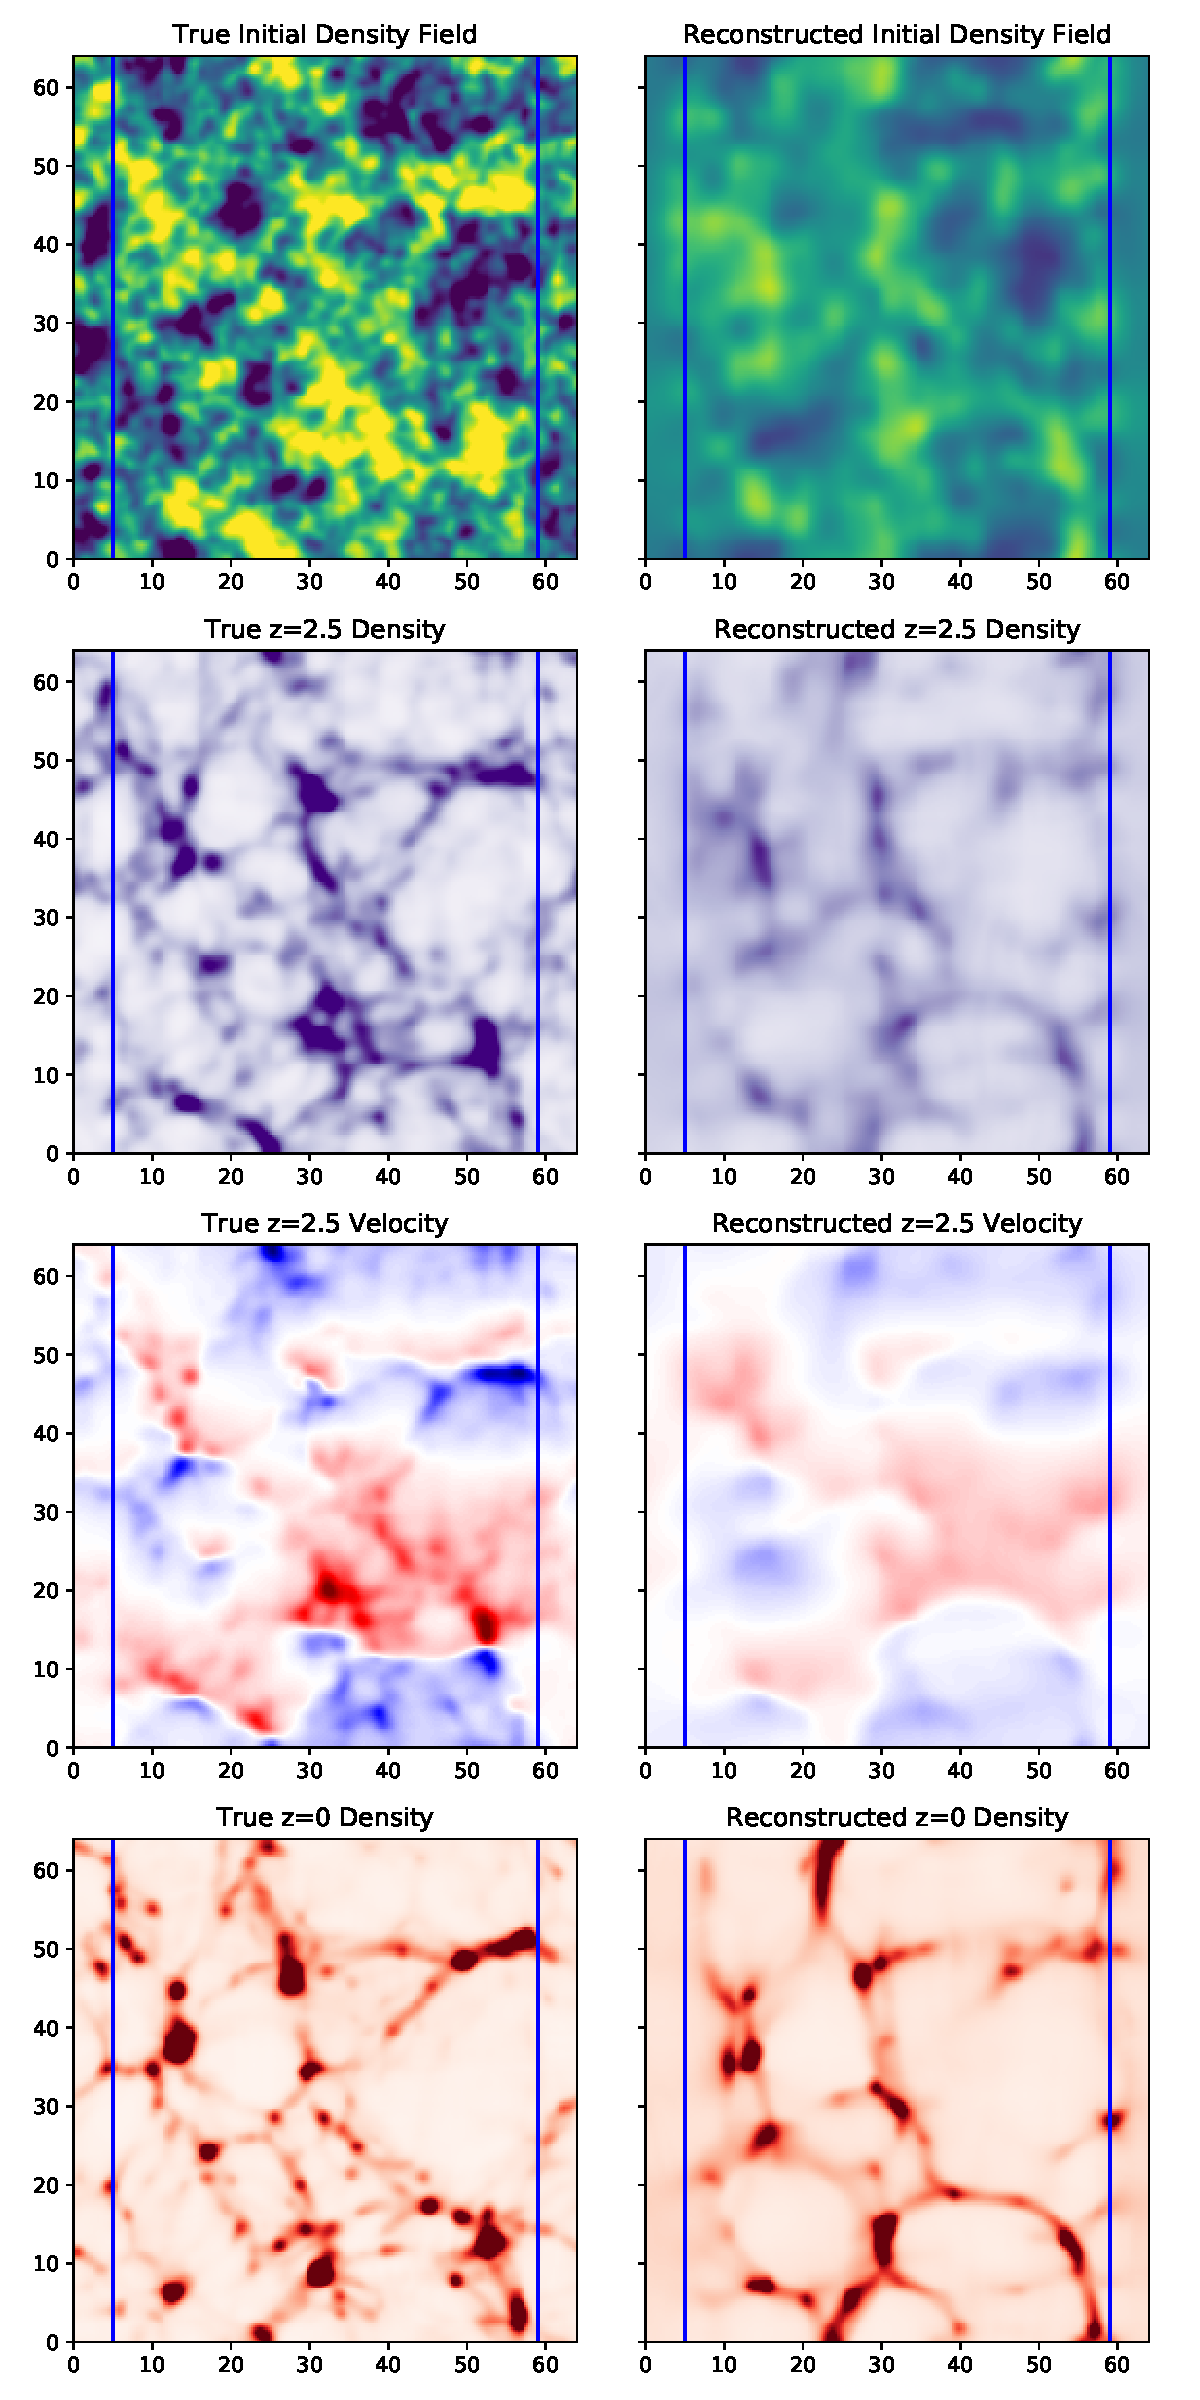
\includegraphics[trim=0cm 0cm 0cm 0cm,width=0.65\textwidth]{./figs_fastpm/8panel.pdf}
    \caption{Plot showing reconstruction of various astrophysical quantities for the \texttt{T-PFS-A} mock dataset.} 
    \label{fig:8panel}
\end{figure}

In addition to the white spectrographic noise we add in a continuum error reflective of the difficulty in identifying the continuum spectrum upon which the Lyman Alpha forest is absorbed. The ability to properly identify the continuum is dependent on the signal to noise of the skewers, and we follow \cite{2018Krolewski} and use a fitted continuum error distribution to apply to our mock skewers. In particular we take our observed flux to be 
\begin{equation}
    F_{\textrm obs} = \frac{F_{\text sim}}{1+\delta_c},
\end{equation}
where $\delta_c$ is taken from an underlying distribution $\sigma_c$ depends on the signal to noise along each skewer as
\begin{equation}
 \sigma_c = \frac{0.205}{{\textrm SNR}} + 0.015
\end{equation}
where the constants are fitted from data from the CLAMATO field. Note that we do not directly address modeling of the spectra continuum in this work beyond this multiplicative error which we assume propagates in an unbiased and uncorrelated way. %The modeling of the continual spectra is itself a rich subject, with active development ... \cite{2017EilersContinua} [more]



\section{Results}

We apply our method, described in \ref{sec:method} to the mock catalogs, described in \ref{sec:mocks} and explore the reconstructed fields. Broadly we are interested in how well we reconstruct cosmic structures both at the observed redshift ($z=2.5$) and the late time ($z=0$) fate of said structures. The overall reconstructed fields for initial density, $z=2.5$ density and flux, line of sight velocity and $z=0$ density for \texttt{T-PFS-A} are shown in Fig \ref{fig:8panel}.

\subsection{Initial Density Field Reconstruction}

The actual accuracy of initial density field is only directly relevant in its effect on late time structures and associated quantities (i.e. velocity fields), however it is useful to 

[pretty picture]

%We also compute the power spectra of our reconstruction. Due to the limited statistics of a single volume we compute the average over 10 volumes. Note, for a more complete power spectra analysis we would need \cite{2018Horowitz}.

\subsection{Matter/Flux Density at $z\sim 2.5$}

As our optimization compares the flux along the line of sight, it is an interesting question as to how well we recover this flux vs. standard $z=2.5$ Wiener filtering techniques which have been standard. As we are assuming the Fluctuating Gunn Peterson approximation, this reconstructed flux can be mapped directly to the density field.


\begin{figure}
  \centering 
  
  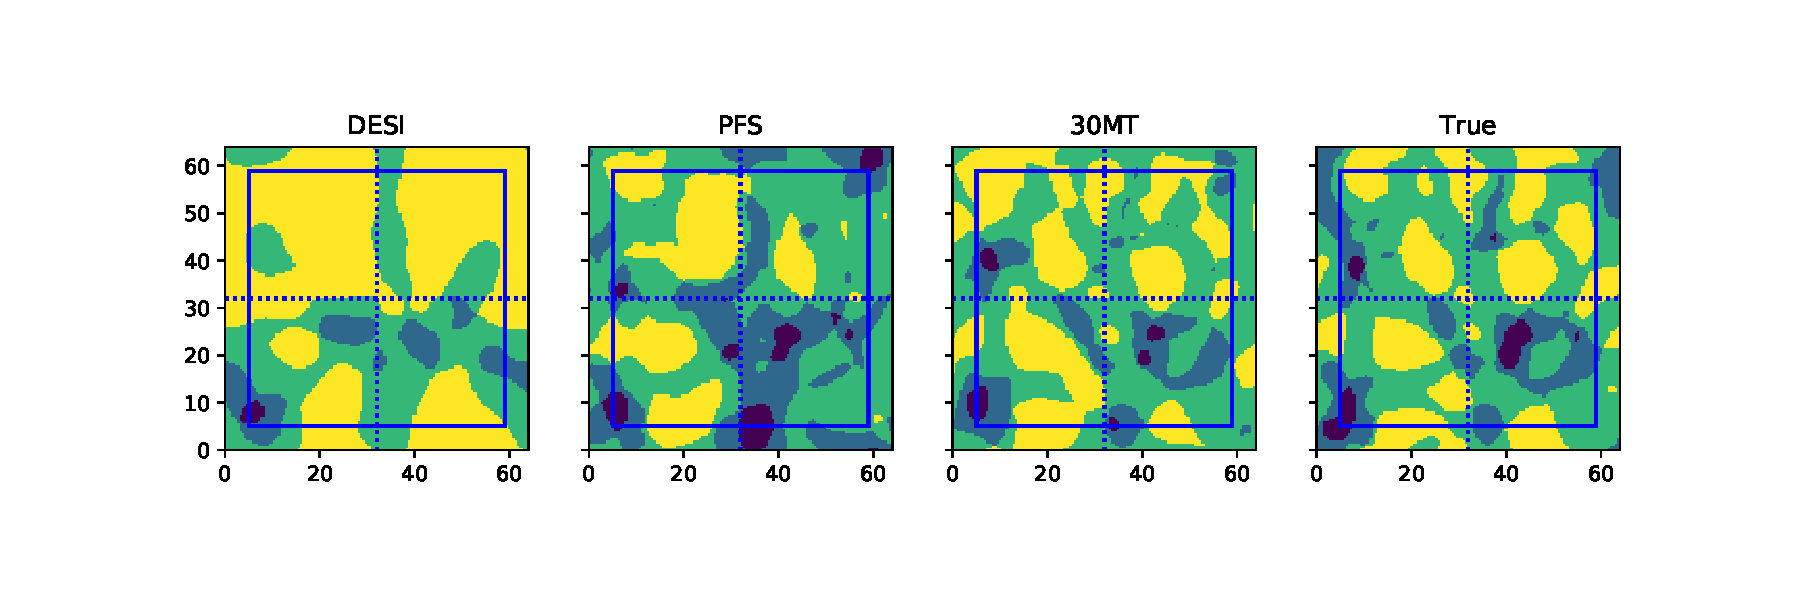
\includegraphics[trim=1cm 2cm 0cm 0cm,width=1.0\textwidth]{./figs_treepm/cosmic_structure_z=2.pdf}
    \caption{Comparison of the z=2.5 reconstructed cosmic structures as classified by their eigenvalues, from \texttt{T-DESI-A}, \texttt{T-PFS-A}, and \texttt{T-30MT-A}, vs. the true z=0 density field. Dark blue indicated node, light blue indicates filament, green indicated sheet, and yellow indicates void.} 
    \label{fig_config}
\end{figure}

\begin{figure}
  \centering 
  
  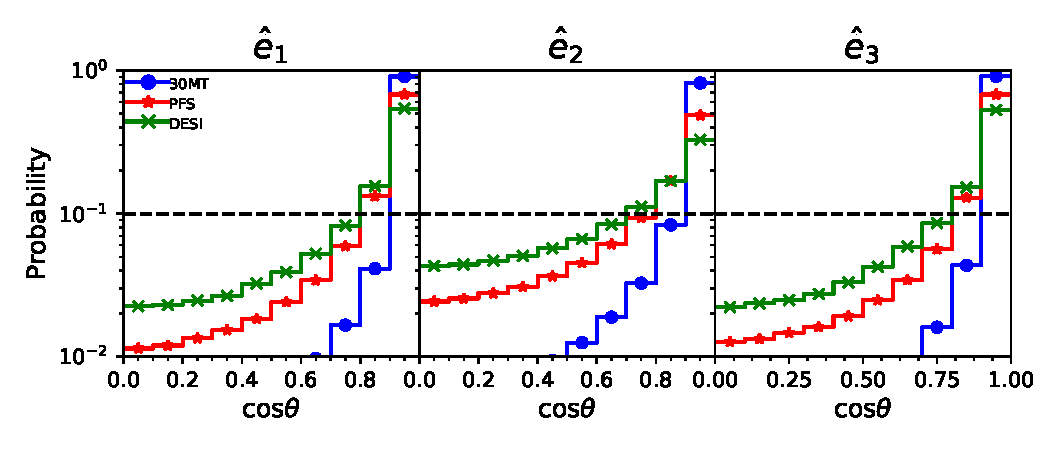
\includegraphics[trim=1cm 0cm 0cm 0cm,width=1.0\textwidth]{./figs_treepm/eigenvectors_z=2.pdf}
    \caption{Showing the dot product of the eigenvectors from cosmic web reconstruction vs. the true cosmic web.} 
    \label{fig_cosmicweb}
\end{figure}

\begin{figure}
  \centering 
  
  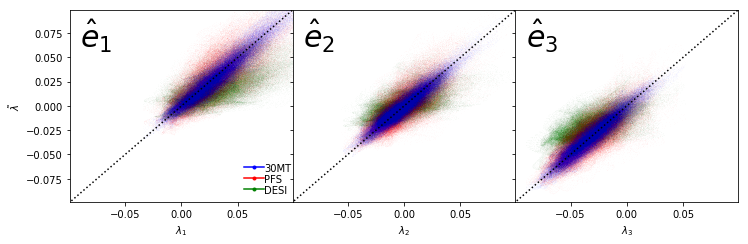
\includegraphics[trim=1cm 0cm 0cm 0cm,width=1.0\textwidth]{./figs_treepm/eigenvalues_z=2.png}
    \caption{Showing the point by point distribution of the eigenvalues inferred from the deformation tensor, smoothing 2 Mpc/h.} 
    \label{fig_eigenvalues}
\end{figure}

\begin{table}
  \begin{center}
    \label{tab:table1}
    \begin{tabular}{c|c|c|c|c|c|c|c} 
    
\multicolumn{8}{|c||}{\textbf{Cosmic Web Reconstruction: z=2.5}}
 \\ 
          \hline
      \hline

& \multicolumn{3}{|c||}{\textbf{Pearson Coefficients}} & \multicolumn{4}{|c||}{\textbf{Volume Overlap}} 
 \\ 
      \hline
      \textbf{Name}& $\hat{e}_1$ &  $\hat{e}_2$ & $\hat{e}_3$ & Node & Filament & Sheet & Void\\
      \hline
      \hline


        \texttt{T-DESI-A} & 0.66 & 0.58 & 0.62 & 28.0 & 52.3 & 58.7 & 44.6\\
        \texttt{T-PFS-A}& 0.77 & 0.75 & 0.78 & 46.5 & 60.1 & 66.2 & 64.6 \\
        \texttt{T-30LT-A} & 0.95 & 0.94 & 0.94 & 75.0 & 80.1 & 82.2 & 79.8\\
    \end{tabular}
        \caption{Pearson correlation coefficients and volume overlap fractions for the three mock datasets, 2 Mpc/h at z=2.5.}

  \end{center}
\end{table}

While in past tomographic maps \cite{Lee2017} have smoothed the field on $1.4$ the sightline spacing, for these comparisons we smooth at 0.75 the sightline spacing in order to compare smaller structures. For example, we expect that the initial density reconstruction method to outperform Wiener filtering at inferring structure between sight-lines as these are where interesting nonlinear and semi-linear structures develop which our method should be able to infer. 

A well-known feature of reconstructed maps are the presence of a bias caused by the presence of noise. We correct for this bias by a linear transformation calibrated from a separate simulated volume. The effect of this transformation is shown in Fig \ref{fig_fluxcompare} (b). 

We show slices for PFS in Fig \ref{fig_wfcompare}. 

We also want to study how well the cosmic web is reconstructed both in terms of orientation and classification of cosmic structures. Using the eigenvectors and eigenvalues of the deformation tensor, Eq. \ref{eq:diften}, we can compare the reconstructed structures to the true structures. Qualitatively, we can see the reconstruction of the cosmic structures in Figure \ref{fig_config}. 

We also examine the eigenvalues in Figure \ref{fig_eigenvalues} and eigenvectors in Figure \ref{fig_cosmicweb}.

\begin{figure}


\begin{center}
\begin{overpic}[width=0.480\textwidth]{./figs_treepm/delta_flux.pdf}
\put(60,-10){\textsf{\scriptsize (a) Pixel flux error}}
\end{overpic}
\vspace{1em}
\begin{overpic}[clip,trim={0cm 0cm 0 0cm},width=0.495\textwidth]{./figs_treepm/scatterplot.pdf}
\put(60,-10){\textsf{\scriptsize (b) Flux reconstruction}}
\end{overpic}
\end{center}

    \caption{Comparing the flux reconstruction for the \texttt{T-PFS-A} mock catalog. For these comparisons we have taken a central box which is $35$ Mpc/$h$ side-length in order to mitigate potential boundary effects and smoothed the region on 1.5 Mpc/h scale. $(a)$ Comparison of the corrected fluxes for the Wiener filter map (see App \ref{app:wf}) and \texttt{TARDIS} reconstruction vs. the true flux. $(b)$ Scatterplot of the \texttt{TARDIS} reconstructed corrected flux vs the true flux. Also shown is the linear fit of the uncorrected flux (dashed grey line) which was linearly transformed to the $x=y$ dotted line. If interpreted as a flux PDF, each level surface indicates $0.5 \sigma$ density.} 
    \label{fig_fluxcompare}
\end{figure}


\subsection{Matter Density at $z =0 $}

The main motivation for the TARDIS framework is inferring the late time fate of structures found in regions observed by Lyman Alpha Tomography. 

\begin{figure}
  \centering  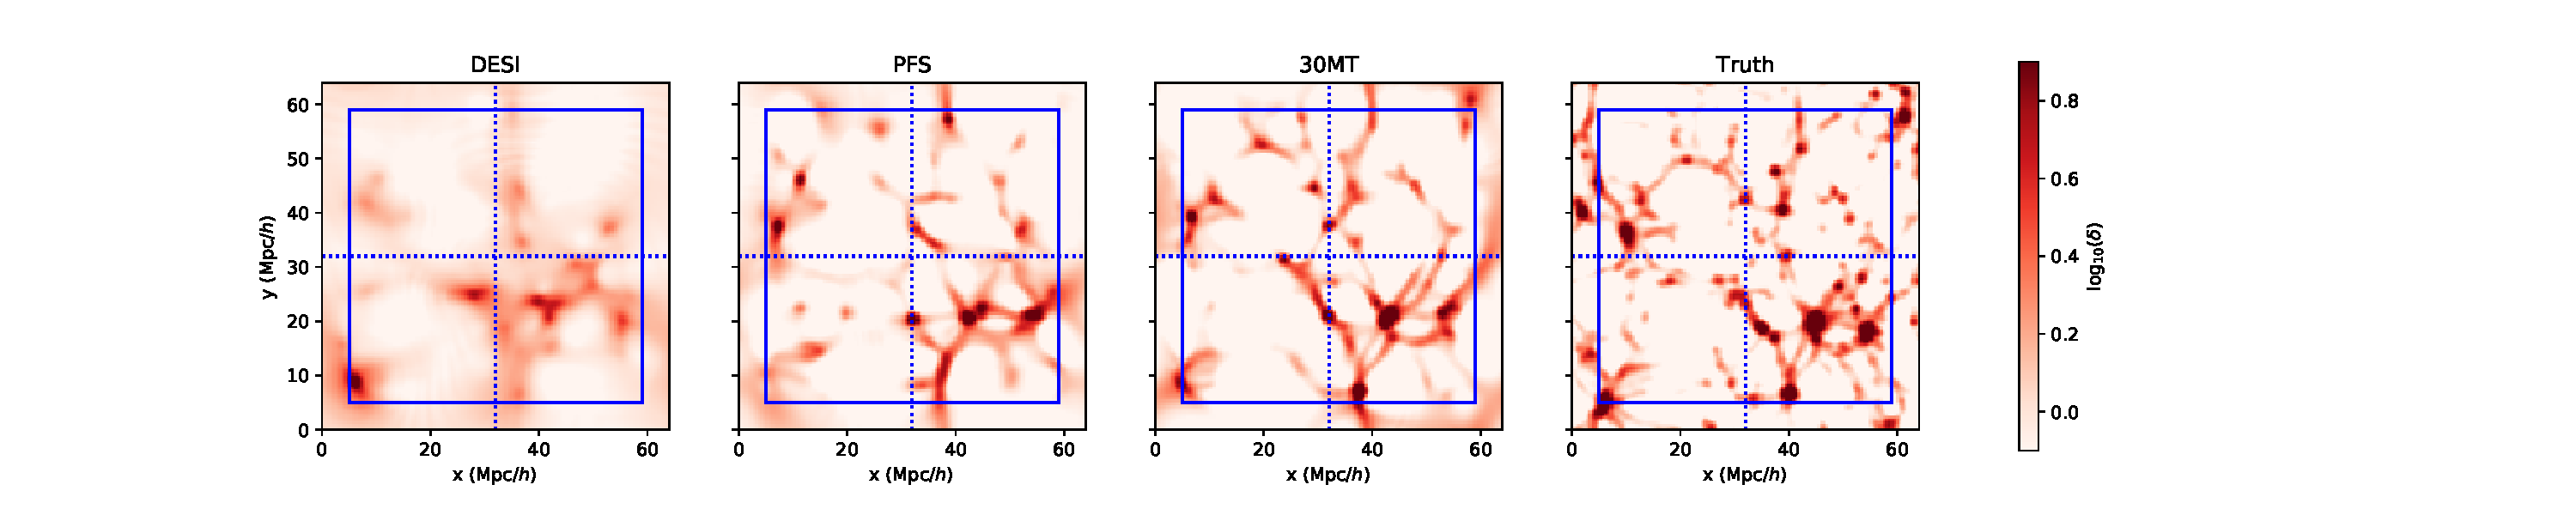
\includegraphics[trim=3cm 0cm 0cm 0cm,width=1.2\textwidth]{./figs_treepm/z=0_density.pdf}
    \caption{Comparison of the z=0 inferred density, from \texttt{T-DESI-A}, \texttt{T-PFS-A}, and \texttt{T-30MT-A}, vs. the true z=0 density field. Projected over 10 Mpc/h thick slice assuming different configurations. Fields have been smoothed at 2 Mpc/h.)} 
    \label{fig_config}
\end{figure}


%\subsection{Velocity at $z\sim 2.5$}

%[s/n-type calculation?]

\section{Discussion}

\section{Conclusion}


We present the first use of initial density reconstruction in the case of Lyman Alpha Tomography, and have showed that using this technique we are able to accurately reconstruct large scale properties within the survey volume over a range of scales.

While we are fundamentally limited by noise levels and sight-line spacing...

In addition, we have shown that the inferred flux maps from this technique are have less scatter compared to those inferred from direct Wiener filtering.

We have demonstrated that it is efficient and practical to [do something]

While only explored indirectly (through $z=0$ density reconstruction) a product of this technique is the particle velocity field at $z=2.5$ which could have signicant uses in informing astrophysical processes as well as cosmological constraints. The velocity field reconstruction extends over the entire field and could be a useful addition beyond velocity fields from galaxy redshift space distortions and kinetic Sunyaev Zeldovich effects.\cite{2017Sugiyama} In addition, this technique would allow reconstruction of void velocity profiles which could provide a constrain on modified gravity \cite{2018Falck} and neutrino mass \cite{2015Massara}.

In this work we have held the astrophysical and cosmological parameters constant. A more complete treatment would require varying these jointly with the underlying field, however we view this as unnecessary at this point since existing data is only over a very limited volume and isn't expected to have any constraining power. For next generation surveys which will greatly expand the footprint covered it will be required to jointly vary these parameters as well. Within the FGPA approximation the astrophysical parameters aren't a significant limitation since there are only a two parameters of interest ($A_0$,$\gamma$) and our optimization scheme is fast enough that a naive Markov Chain Monte Carlo sampling would be sufficient to explore this parameter space. We explore the sensitivity of the reconstruction on the absorption model in Appendix \ref{app:sens}.

Our focus in this work was on reconstructing the large scale structure within the survey volume, finding we were able to recover qualitative structure over a range of scales. Going forward, it would be useful to study how well similar techniques would be on reconstructing halo-scale (i.e.  $\leq 1$ Mpc) structure, such as halo and void profiles. However, going to this small scale regime reconstruction will be limited by the the specific astrophysical processes within the cluster where the Fluctuating Gunn Peterson Approximation will no longer hold. It should be possible to extend the formalism proposed in this work and treating the variations from FGPA as a biased tracer, with some additional parameters to be fit for (or marginalized) in this limit, such as was done for galaxy surveys in \cite{2015ata,2016Kitaura,2018BORG}. One could also use grid-based approximation methods for bayronic effects (such as \cite{2018Dai}) to provide a more precise formalism for halo substructure. It would be a natural extension to test this method on mock data generated from the NyX hydrodynamic simulations designed to emulate Lyman Alpha absorption physics \cite{2013nyx,2015nyxlya}.

On the other side, additional work would be needed to make this reconstruction technique useful for full scale cosmological analysis. Directly extracting power power-spectra estimates from our reconstructed maps suffers from significant noise bias effects which would make them difficult to apply directly to constrain cosmological parameters, as well as complicated mode coupling effects due to the complexity of our forward model. Using a response formalism (as in \cite{seljak2017towards,2018Horowitz,2018fengseljakzaldarriaga}) to estimate band-powers would be straightforward and would require $O(N)$ additional optimization runs to estimate $N$ band-powers. However, before trusting such reconstruction for cosmological analysis additional considerations are necessary, such as adjusting for light-cone effects (i.e. evolution) within the survey volume and incorporation of correlated error. Work in this direction is ongoing.



\section*{Acknowledgments}
We appreciate helpful discussions with Uro${\rm \check{s}}$ Seljak, Yu Feng, and ... 
BH is supported by the NSF Graduate Research Fellowship, award number DGE 1106400, and by JSPS via the GROW program.

This research used resources of the National Energy Research Scientific Computing Center, a DOE Office of Science User Facility supported by the Office of Science of the U.S. Department of Energy under Contract No. DE-AC02-05CH11231.

\appendix


\section{Convergence}

An important question with any optimization scheme is the convergence properties of the procedure. This is particularly important for nonlinear processes like structure evolution where the likelihood surface is non-Gaussian and conceivably non-convex. We divide the issue into two questions to explore in this appendix; how many iterations are necessary for to be confident in our reconstruction technique and how sensitive is the found solution to the initial optimization starting point? For both these questions we explore both the overall quality via the signal-to-noise calculation \cite{2014LeeObserving} as well as a function of scale by looking at the transfer function.
 
It has been shown that at the very low noise limit the likelihood surface of possible initial conditions in multi-modial; i.e. that gravitational evolution is a non-injective map from initial conditions to late time structure.\cite{2018fengseljakzaldarriaga} However, this uncertainty is due to shell-crossing degeneracy which is only relevant for small scale non-linear structure which isn't observed by even the optimistic configurations considered in this work due to spectrographic smoothing, sight-line density and noise levels. To study whether or not there is one "true" solution or if there exist sufficiently different converged solutions we perform the optimization analysis for the same mock catalog with different optimization starting points. In particular, we randomly choose starting points white noise maps with amplitudes spanning 3 orders of magnitude. We plot their transfer functions after 100 iterations vs. a fiducial ``well-converged" solution which underwent 500 iteration steps, in Figure \ref{appfig_startingpoints}. Note that we don't compare against the true power-spectra since there are substantial noise bias contributions which make such a comaprison difficult. In the scales of interest for the structures studied in this work, $\approx 1$ Mpc/h we find very close agreement between all different starting points. 

There is some significant differences of power at very large scales, reflective of the poor constraining power of modes of order the box-size. The number density of modes per uniform bin scales as $k^2$ resulting in significantly more weight getting placed on smaller modes, up till the window function (depending on the smoothing scale and sight-line density) creates a sharp cutoff. If these larger modes are of significant interest, an adiabatic optimization scheme could be used where-in the optimization begins first on a smoothed version of the observed field and then slowly small scale power is introduced back in by varying the smoothing scale as the optimization progresses (as done in \cite{2018fengseljakzaldarriaga}), or potentially directly using a multi-grid preconditioner technique.\cite{2007multigrid} Utilization of these techniques will likely be useful when extending this work for cosmological analysis.

The next important consideration is how long our scheme takes to be fully converged.

By $n=100$ we find good agreement up to $k = 1.0$ Mpc/h, justifying our use of this criteria in the main work.


\begin{figure}
  \centering  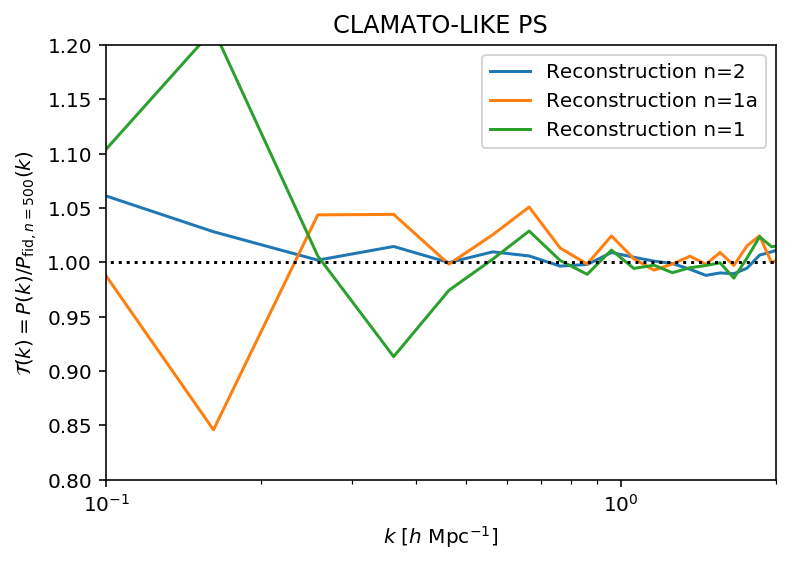
\includegraphics[trim=0cm 0cm 0cm 0cm,width=0.90\textwidth]{./appendix_figures/different_starts.png}
    \caption{\texttt{T-CLAMATO} Transfer function of various solutions with different starting points. [Temporary Figure]} 
    \label{appfig_startingpoints}
\end{figure}



\begin{figure}
  \centering  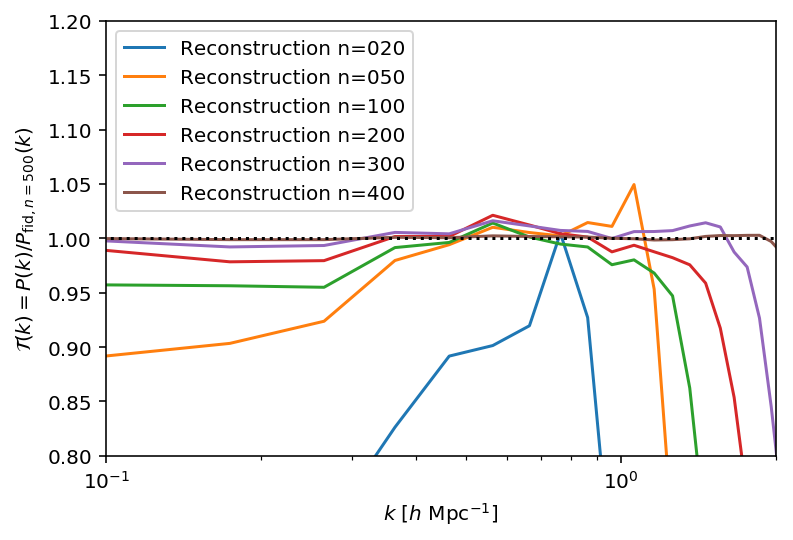
\includegraphics[trim=0cm 0cm 0cm 0cm,width=0.90\textwidth]{./appendix_figures/transfer_iterations.png}
    \caption{\texttt{F-IDEAL} Power Spectra convergence. [TEMPORARY FIGURE]} 
    \label{fig_sims2x2}
\end{figure}


\begin{figure}
  \centering  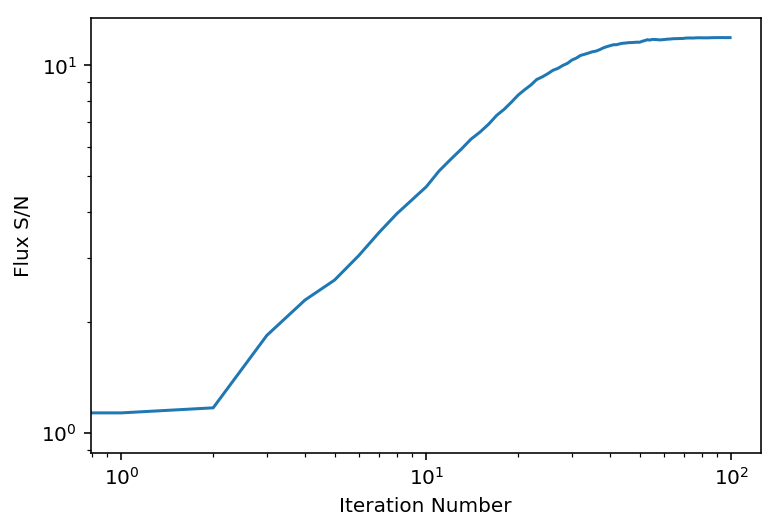
\includegraphics[trim=0cm 0cm 0cm 0cm,width=0.90\textwidth]{./figs_fastpm/flux_sn.png}
    \caption{CLAMATO-like MOCK (FASTPM) S/N over iteration number} 
    \label{fig_sims2x2}
\end{figure}




\section{Sensitivity to Cosmology and Absorption Model}
\label{app:sens}

In the main body of this work we have held cosmological and astrophysical parameters constant for the reconstructions. Here we briefly explore how wrong assumptions about the astrophysics or cosmology would bias our late time density field. 

We use a different mock catalog, \texttt{T-IDEAL}, in order to examine the effects of varying the astrophysical parameters. This catalog has a constant signal to noise of $50$ along each skewer, no continuum error, and a sightline density twice that of \texttt{T-30MT-A}. The idea of this super-experiment is to isolate the effects of the astrophysics from other potential sources of noise in the reconstruction.

\begin{figure}
\centering 
 % 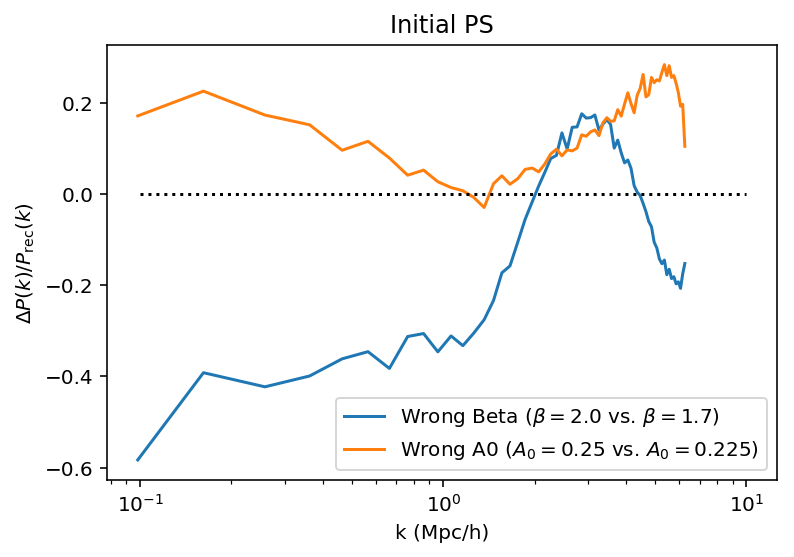
\includegraphics[trim=0cm 0cm 0cm 0cm,width=0.70\textwidth]{./appendix_figures/absorp_initial.png}
  
  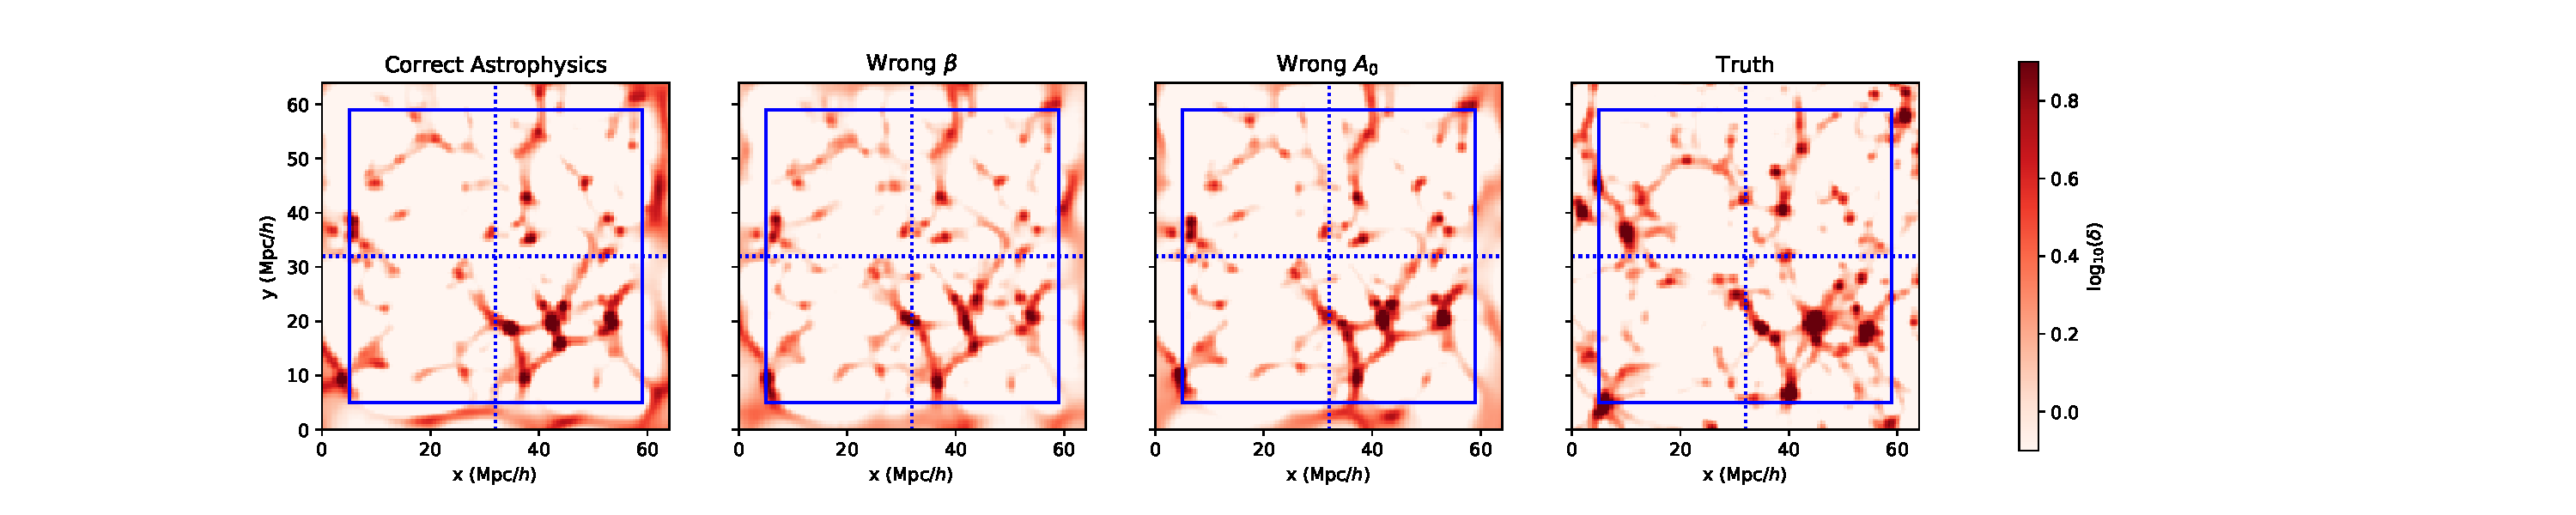
\includegraphics[trim=3cm 0cm 0cm 0cm,width=1.2\textwidth]{./appendix_figures/z=0_wrongdensity.pdf}
  
  
  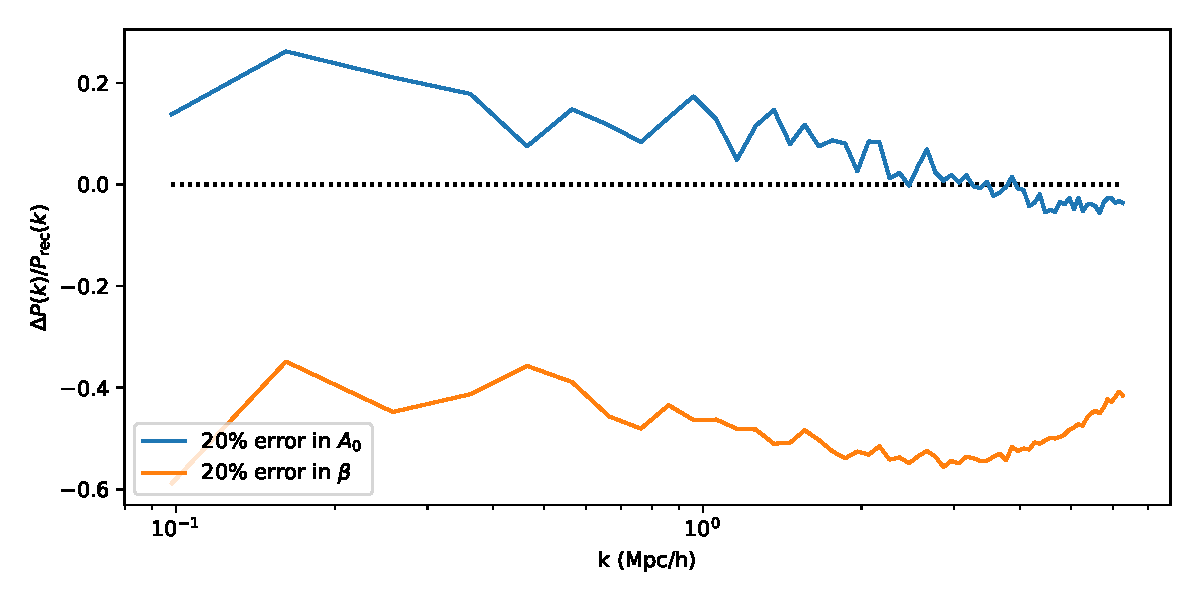
\includegraphics[trim=0cm 0cm 0cm 0cm,width=0.70\textwidth]{./appendix_figures/wrong_astro_ps.pdf}
    \caption{Effect of assuming the wrong astrophysical parameters on the z=0 structure, both for a slice in real space and the power spectra} 
    \label{fig_sims2x2}
\end{figure}

In practice, for surveys of the size studied in this work, it would be easily numerically tractable to sample over these parameters to perform the late time reconstruction or, alternatively, to use Lyman Alpha Tomography as a constraint on these parameters.



\section{Comparison to Wiener Filtering}
\label{app:wf}

A promising aspect of this initial density reconstruction technique is that the reconstructed $z\sim 2$ flux field should be strictly more accurate than that from direct wiener filtering (WF) of the skewers. This is because direct WF is a purely statistical process which does not take into account the physical evolution of the system under gravity which further constrains the observed flux field. In this section we review the WF technique which we compare our method against. For a more general discussion of efficient WF and associated optimal bandpower construction, see \cite{seljak1998cosmography,2018Horowitz}. For a more through description in the context of Lyman alpha forest, see \cite{Stark2015}.

As we are trying to reconstruct the optimal map given the data, we have to take into account both the data-data covariance, $\textbf{C}_{\textrm{DD}}$, the map-data covariance, $\textbf{C}_{\textrm{MD}}$, and the overall noise covarance, $\textbf{N}_{ij}$. The reconstructed map can then be expressed in terms of the observed flux, $\delta_F$ as a standard Wiener filter by ;

\begin{equation}
\delta_F^{\textrm{rec}} = \textbf{C}_{\textrm{MD}} \cdot
(\textbf{C}_{\textrm{DD}} + \textbf{N})^{-1} \cdot \delta_F.
\label{eqn:wiener}
\end{equation}
Approximate covariance with lots of assumptions... In the absence of continuum or other correlated errors, $\textbf{N}_{ij}
= n_i^2 \delta_{ij}$ where $n_i$ is the pixel noise.
\begin{equation}
C = \sigma_F^2 \exp{\left[-\frac{\Delta x_{\perp}^2}{2 l_{\perp}^2}
- \frac{\Delta x_{\parallel}^2}{2 l_{\parallel}^2}
\right]}
\label{eqn:covariance}
\end{equation}




\begin{figure}

  \centering  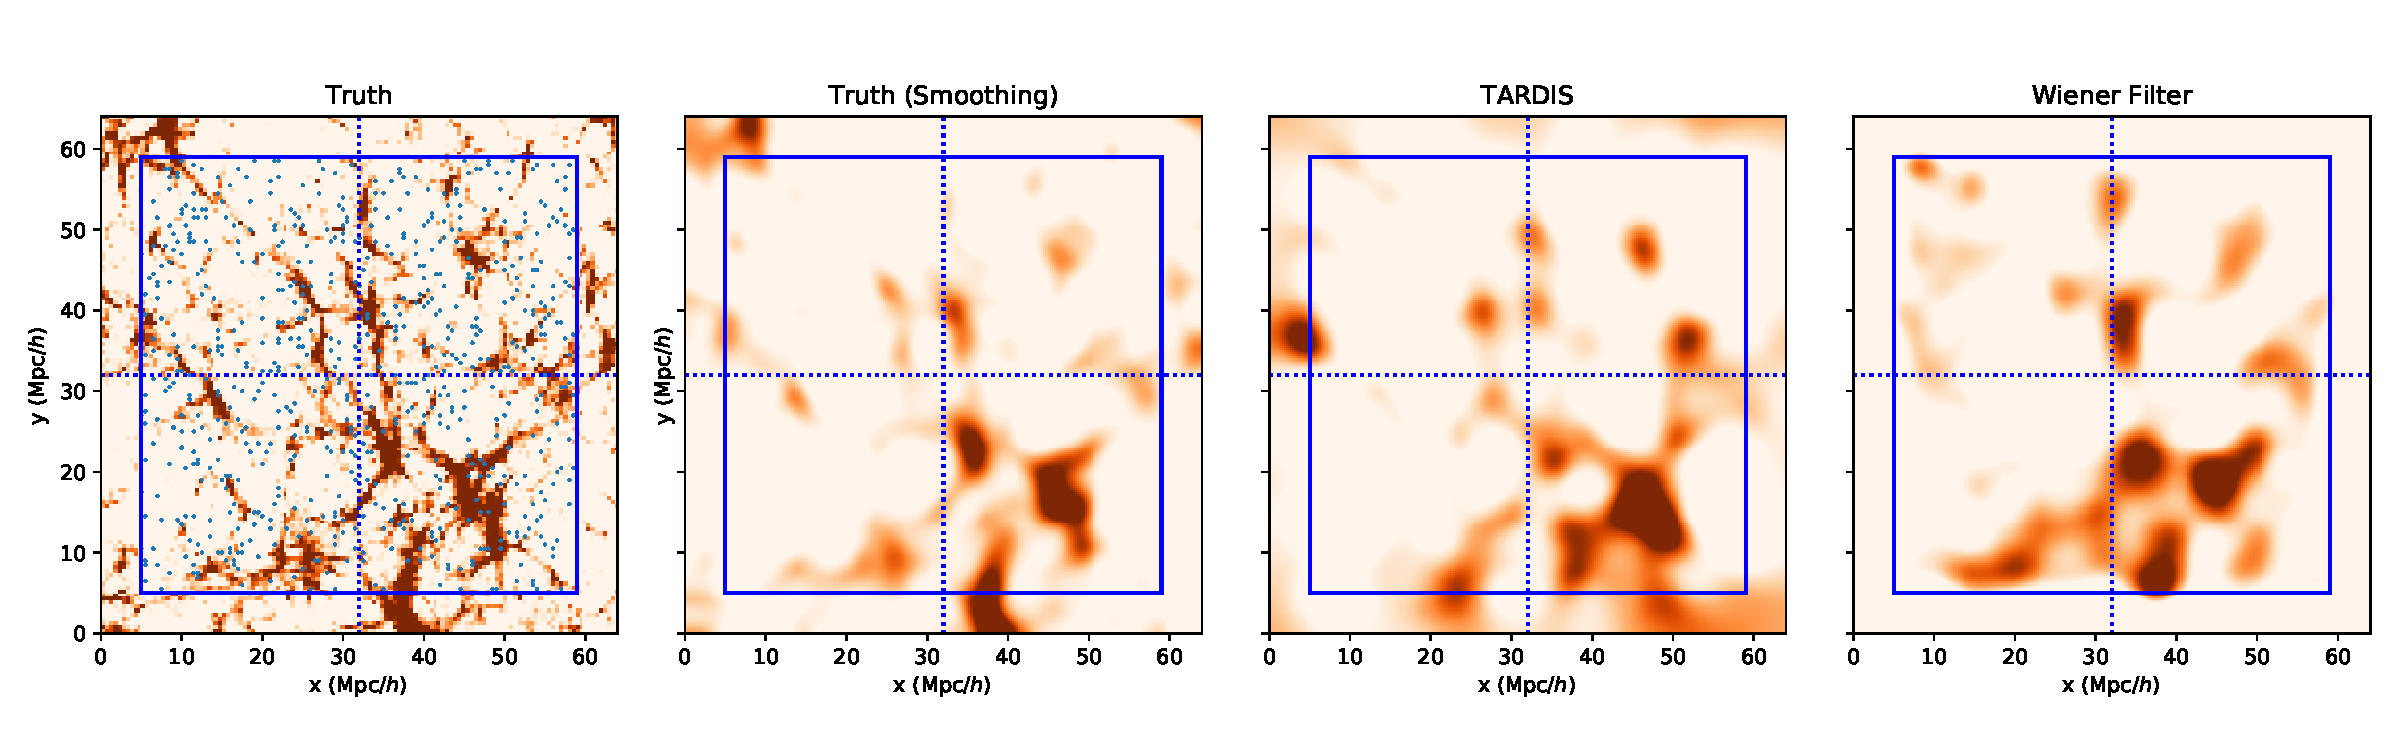
\includegraphics[trim=0cm 0cm 0cm 0cm,width=0.80\textwidth]{./figs_treepm/wf_comparison/wf_compare_pfs14.pdf}
  \centering  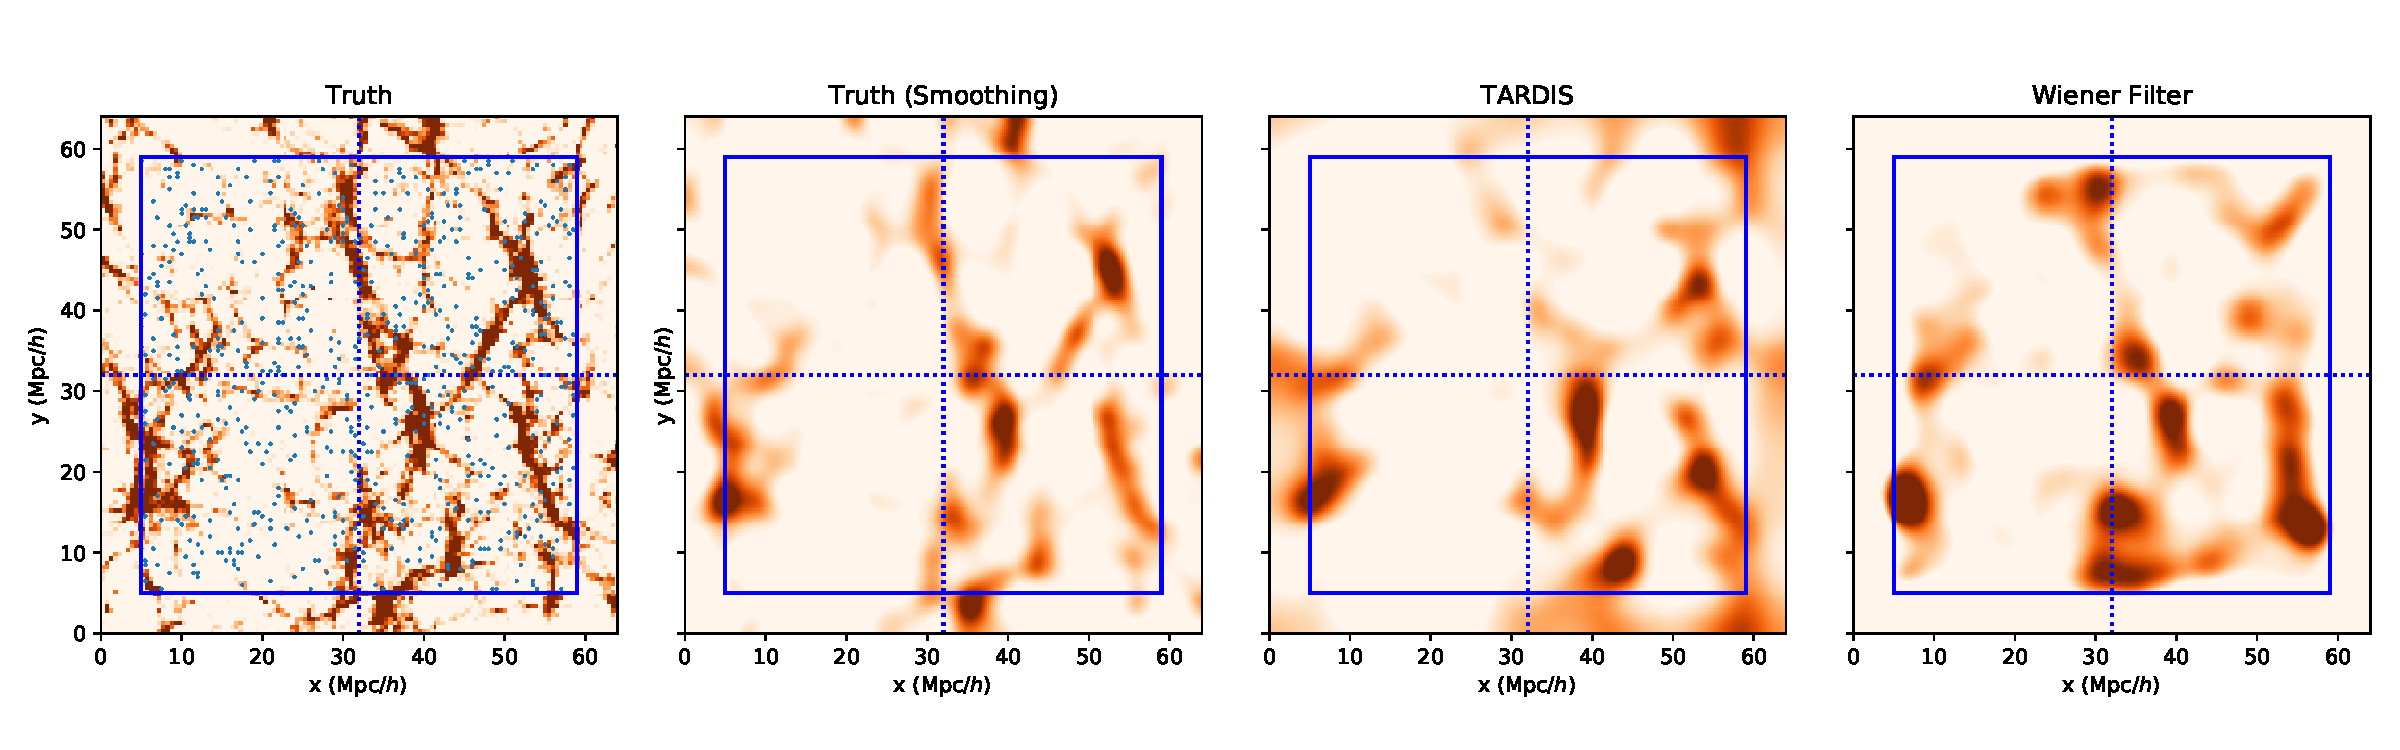
\includegraphics[trim=0cm 0cm 0cm 0cm,width=0.80\textwidth]{./figs_treepm/wf_comparison/wf_compare_pfs64.pdf}
  \centering  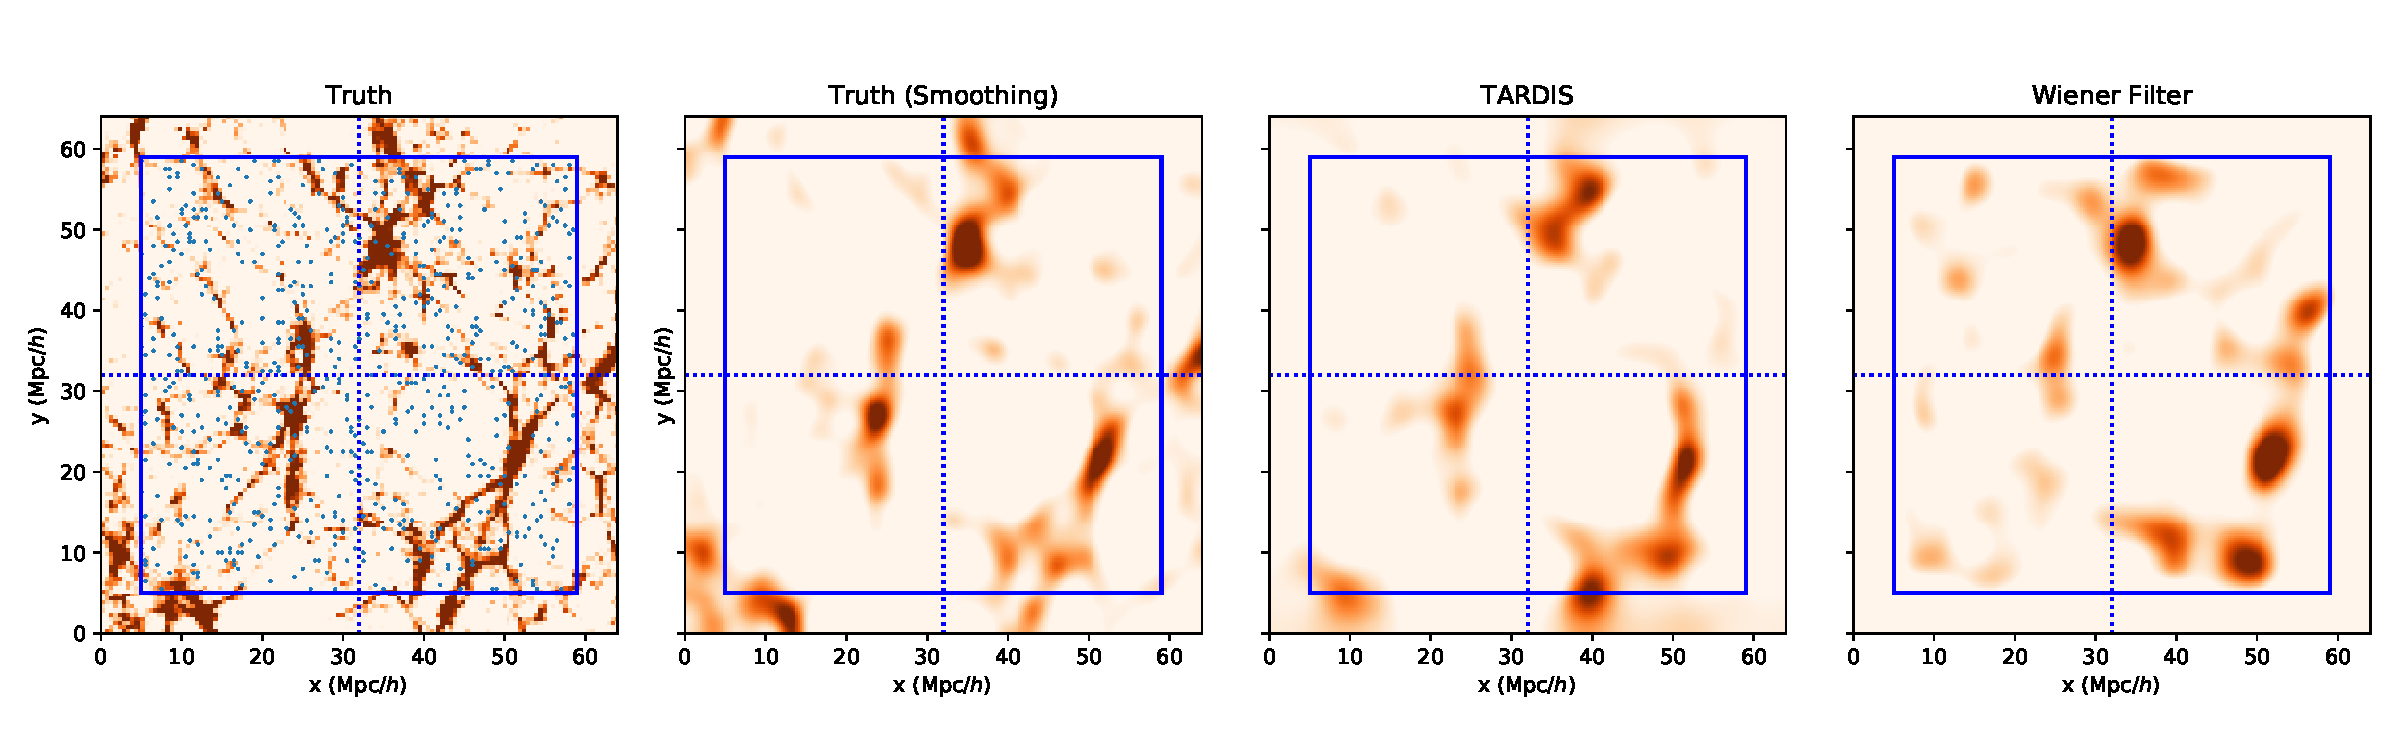
\includegraphics[trim=0cm 0cm 0cm 0cm,width=0.80\textwidth]{./figs_treepm/wf_comparison/wf_compare_pfs114.pdf}
    \caption{Comparison of the true field, \texttt{TARDIS} reconstructed field, and the wiener filtered field for the \texttt{T-PFS-A} mock. In the far left panels we show the unsmoothed true flux field, with sightlines indicated as blue dots. The blue box indicates boundaries of the survey, with the blue cross to help aid the eye in matching structures. We smooth the 3 rightmost column maps on a 1.5 Mpc/h and project over a 5 Mpc slice.} 
    \label{fig_wfcompare}
\end{figure}


\bibliographystyle{mnras}

%\bibliographystyle{unsrt}
\bibliography{sample}

\end{document}